\section{Påverkande faktorer}
Reaktionshastigheten kan påverkars av många faktorer\footnote{se s. 28--31 i boken}. Här kommer en sammafattning.
\subsection{Bindningar}
Fria joner reagerar nästa omedelbart, exempelvis i fällningar. När detta sker är reaktionen \emph{momentan}. Fri joner har inte några bindningar som måste brytas innan reaktionen kan ske vilket gör det snabbare. Molekyler kommer alltid att reagera långsammare då det tar tid och energi att bryta deras bindningar för reaktionen.

\subsection{Kontaktyta}
Jo större ytan som reaktionen sker på är desto snabbare kommmer den att gå. Detta beror på att de reagerande ämnena måste kollidera för att reaktionen ska ske. Ju mer yta att kollidera på desto fler kollisioner alltså desto snabbare reaktion.

\subsection{Aggregationstillstånd}
Aggregationstillståndet, eller i detta fall hur fritt partiklarna rör sig, kommer ha en stor effekt på reaktionshastigheten. En gas kommer ju ha högst rörlighet, sedan vätskor och sist fasta ämnen. Ju mer partiklarna rör sig desto fler chanser kommer de få att kollidera med varandra och desto snabbare kommer reaktionen att gå.

\subsection{Katalysatorer}
\label{sec:katalysator}
En katalysator är ett ämne som gör en reaktion snabbare eller möjliggör en reaktion som annars är omöjlig utan att själv förbrukas. Den gör detta genom att sänka aktiveringsenergin (se \vref{sec:entalpiaktiveringse})av reaktionen. Antingen kommer den att hamna under gränsen för tillgänglig energi vilket möjliggör reaktionen eller så kommer den helt enkelt minska energikravet och öka hastigheten.

\subsection{Koncentration}
En högre koncentration gör partiklarna tätare vilket i sin tur leder till snabbare reaktioner. Detta medför också att tryckförändringar påverkar reaktionshastighet i komprimerbar materia (ex. gaser).

\section{Reaktionens energi}

\subsection{Endoterm och exoterm}
En reaktion kan vara endo- eller exoterm. En endoterm reaktion kräver energi medan en exoterm reaktion avger ett överskott av energi\footnote{se s. 32--33 i boken}.

\subsection{Entalpi och aktiveringsenergi}
\label{sec:entalpiaktiveringse}
\begin{figure*}[h]
    \centering
    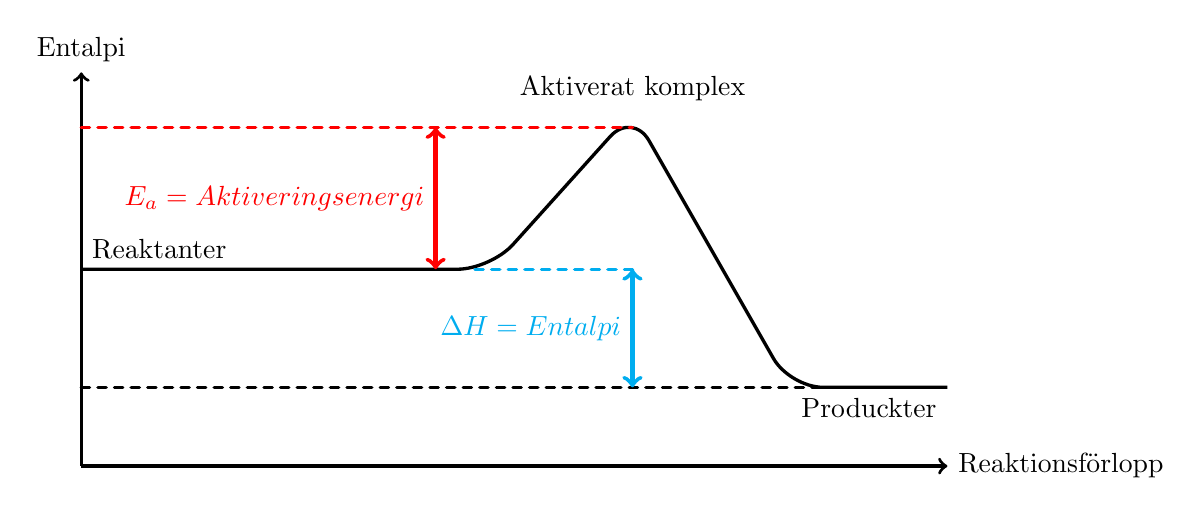
\begin{tikzpicture}
        \draw [->,very thick] (0,0) -- (0,5) node[anchor=south] {Entalpi};
        \draw [->,very thick] (0,0) -- (11,0) node[anchor=west] {Reaktionsförlopp};
        \draw [very thick,rounded corners=12pt] (0,2.5) node[anchor=south west] {Reaktanter} -- (5.2,2.5) -- (7, 4.5) node[anchor=south] {Aktiverat komplex} -- (9,1) -- (11,1) node[anchor=north east] {Produckter};
        \draw [dashed,very thick,color=red, line cap=round] (0,4.3) -- (7,4.3);
        \draw [dashed,very thick, line cap=round] (0,1) -- (10.5,1);
        \draw [ultra thick,<->,color=red] (4.5,2.5) -- (4.5,3.4) node[anchor=east] {$E_a = \text{Aktiveringsenergi}$} -- (4.5,4.3);
        \draw [very thick, dashed, color=cyan, line cap=round] (5,2.5) -- (7,2.5);
        \draw [ultra thick, <->, color=cyan] (7,1) -- (7,1.75) node[anchor=east] {$\Delta H =\text{Entalpi}$} -- (7,2.5);
    \end{tikzpicture}
\end{figure*}

\noindent Denna graf visar förloppet av en reaktion uttryckt som energiförändring över tid. Energin är mätt i enheten $\mathrm{kJ/mol}$ som på sätt och vis uttrycker energikoncentration baserat på substansmängd vilket kallas \emph{entalpi}\footnote{se s. 32--36 samt uppgift 2:11 i boken}. När man säger entalpi menar man ofta förändringen i entalpi som uttrycks $\Delta H$. Detta visar om det har avgetts eller absorberats energi under reaktionens gång:
\begin{align*}
    \Delta H < 0 &\Rightarrow \text{exoterm reaktion, energi avges} \\
    \Delta H > 0 &\Rightarrow \text{endoterm reatkion, energi absorberas}
\end{align*}

På grafen kan vi även den så kallade \emph{aktiveringsenergin} $E_a$. Denna energi är är skillnaden mellan den ursprungliga energinivån av reaktanterna och den mängd energi som krävs för att reaktionen ska ske. Man kan resonera kring aktiveringsenergi från båda hållen i diagrammet. Just nu finns bara det högra hållet inritat, men i jämvikter går ju det åt båda håll och därmed finns det värde även i produkt $\rightarrow$ reaktant resonemanget.